% !TeX root = ../main.tex
% Add the above to each chapter to make compiling the PDF easier in some editors.

\newcommand{\twopartdef}[4]
{
	\left\{
	\begin{array}{ll}
		#1 &  #2 \\
		#3 &  #4
	\end{array}
	\right.
}

\newcommand*\interior[1]{#1^{\mathsf{o}}}

\newcommand*{\QEDA}{\hfill\ensuremath{\blacksquare}}%

\newcommand{\tab}[1]{\hspace{.1\textwidth}\rlap{#1}}

\newenvironment{tightcenter}{%
	\setlength\topsep{0pt}
	\setlength\parskip{0pt}
	\begin{center}
	}{%
	\end{center}
}

\epstopdfDeclareGraphicsRule{.tif}{png}{.png}{convert #1 \OutputFile}
%\AppendGraphicsExtensions{.tif}

%\newcommand*{\txtspc}[1]{\phantom{.}#1\phantom{.}}%

\chapter{Problem Analysis and Controller Design}\label{chapter: theory}

\section{Stability of Coverage Control}
From (\ref{optimal_comndition}), we have
\begin{equation} \label{primitive_time_derivative_cost_function}
\begin{split}
\dot H(Z) & = \displaystyle\sum_{k=1}^{n}\frac{\partial H(Z)}{\partial {z_k}} \dot{z_k} \\
& = \displaystyle\sum_{k=1}^{n} M_{V_{k}}\langle{z_{k} - C_{V_{k}},\dot{z}_k}\rangle \\
\end{split}
\end{equation}

\noindent By designing a proper feedback control law, we can ensure the time derivative of coverage cost function to be negative and therefore the coverage control is asymptotic stable. In [1], Liu already implemented a control strategy that satisfies the above-mentioned condition. By using this controller, WMR can change its heading orientation and keep moving forwards to orbit any arbitrary center points. 
\begin{equation}\label{control_no_constraint}
u_{k} = w_{k_0} +  \gamma_{k} w_{k_0} \langle{z_{k} - C_{V_{k}},v_{k}e^{i\theta_{k}}}\rangle \\ % <z_{k} - C_{V_{k}}, v_{k}e^{i\theta_{k}}> 
\end{equation}
\noindent where 
\[\gamma_{k} \in \mathbb{R}_+\] 
\[C_{V_{k}} \in \mathbb{C} \txtspc{,} C_{V_k} = C_{kx} \txtspc{+} iC_{ky} \] 
\textbf{Proof.}
\begin{equation} \label{design_z}
\begin{split}
(\ref{VM_dynamic}),(\ref{control_no_constraint}) & \implies  \dot z_k = -\gamma_k v_k e^{i\theta_{k}} \langle{z_k - C_{V_{k}},v_k e^{i\theta_{k}}}\rangle \txtspc{,} \gamma \in \mathbb{R}_+  \\
\end{split}
\end{equation}

\noindent Substitute (\ref{design_z}) into (\ref{primitive_time_derivative_cost_function})
\begin{equation} \label{non_negative_H(Z)}
\dot H(Z) = - \gamma_k M_{V_k}\langle{z_k - C_{V_{k}}, v_{k}e^{i\theta_{k}}}\rangle^2 \leq 0
\end{equation}

\noindent The time derivative of ${H(Z)}$ is always non-positive and is equal to zero only when the virtual mass converge to the centroidal of the Voronoi partition. The asymptotic stability of the coverage problem motivates us to design a controller according to the non-negativity of ${H(Z)}$ from (\ref{design_z}) and the dynamic of virtual mass from (\ref{VM_dynamic}).


\noindent However, the stability of the coverage control is only guaranteed whenever the rotation velocity is feasible. Because of the input constraints, the control law from (\ref{control_no_constraint}) might saturate and impair the negativity of $H(Z)$. In the next part, we analyze the behavior of the proposed control method to determine potential issues caused by the input saturation. Afterwards, a modified control method is proposed to overcome the problem. The following derivation will point out the reasons that trigger input saturation and propose a method to overcome it. 

\section{Problem of Input Constraint}
Recall the control strategy from (\ref{control_no_constraint})
\begin{figure}[h]
	\centering
	\includegraphics[width=0.8\textwidth]{Psi_illustration}
	\caption{Illustration of ${\psi_{k}}$}
	\label{fig:control_input_constraint}
\end{figure}

%\[u_{k} = w_{0} + \gamma_{k} w_{0}v_{k}[(z_{kx} - C_{kx})cos(\theta_{k}) + (z_{ky} - C_{ky})sin(\theta_{k})]\] 
%\[u_{k} = w_{k_0} +  \gamma_{k} w_{k_0} \langle{z_{k} - C_{V_{k}},v_{k}e^{i\theta_{k}}}\rangle\] 
\noindent We reformulate the control law from (\ref{control_no_constraint}) as
\[u_{k} = w_{k_0} + \gamma_{k} w_{k_0} v_{k}\norm{z_{k} - C_{V_{k}}}cos(\psi_{k})\]

\noindent where
\[\gamma_{k} \in \mathbb{R}_+\]
\[w_{k_0}, v_{k} = const \txtspc{,} v_k \in \mathbb{R}_+\]
\[\psi_{k} = \angle (z_{k} - C_{V_{k}}, v_{k}e^{i\theta_{k}})\]  

\noindent Figure \ref{fig:control_input_constraint} depicts the relation between desired control input and actual state of each WMR. We observe that the norm of control input depends on two factors: \\ \\
\indent $\bullet$ ${d_{k}(z_{k}) = \norm{z_{k} - C_{V_{k}}} = \sqrt{(z_{kx} - C_{kx})^{2} + (z_{ky} - C_{ky})^{2}}}$ \\
\indent $\bullet$ ${cos(\psi_{k}) \txtspc{,} \psi_{k} = \angle ({z_{k} - C_{V_{k}}},{v_{k}}e^{i\theta_{k}})}$  \\

%\noindent We can avoid control input saturation by using an adaptive control gain parameter ${\mu_{k}(\psi_{k})}$, which prevents ${u_{k}}$ from reaching its limits. As long as the control input is feasible, the time derivative of cost function is guaranteed to be non-positive as shown in (\ref{non_negative_H(Z)}).\\

\noindent \textbf{Proposition 1:} \\
\noindent By using the following control law, there always exist a positive control gain ${\mu_k(\psi_k)}$ for all agent that make the their virtual masses converge the set of centroidal Voronoi configuration and always satisfies the feasibility of control input.
\begin{equation} \label{control_with_consraint}
\txtspc{ } u_{k} = w_{k_0} + \mu_k(\psi_{k})sign(w_{k_0})cos(\psi_{k})\txtspc{,} \mu_k(\psi_{k}) \in \mathbb{R}_+ \\
\end{equation}
\noindent \textbf{Proof.} \\
$\bullet$ \textit{Asymptotic Stability of Coverage Control} \\
\noindent With the proposed controller in (\ref{control_with_consraint}), the dynamic of virtual mass ${z_k}$ from (\ref{VM_dynamic}) is\\
\begin{equation}  \label{vm_dynamic_with_controller}
\begin{split}
\dot z_{k} & =  (v_k - \frac{v_k}{w_{k_0}}u_k)e^{i\theta_{k}} \\
& = -\mu_k(\psi_{k})\frac{v_k}{\norm{w_{k_0}}} cos(\psi_{k})e^{i\theta_{k}} \\
\end{split}
\end{equation}

\noindent Substitute (\ref{vm_dynamic_with_controller}) into (\ref{primitive_time_derivative_cost_function})
\begin{equation}\notag
\begin{split}
\dot H(Z) & = \displaystyle\sum_{k=1}^{n} M_{V_{k}}\langle{z_{k} - C_{V_{k}},\dot z_k}\rangle \\
& = \displaystyle\sum_{k=1}^{n} M_{V_{k}}\langle{z_{k} - C_{V_{k}},-\mu_k(\psi_{k})\frac{v_k}{\norm{w_0}} cos(\psi_{k})e^{i\theta_{k}}}\rangle \\
& = - \displaystyle\sum_{k=1}^{n} \frac{\mu_k(\psi_{k})M_{V_{k}}v_{k}}{\norm{w_{0}}} \langle{z_{k} - C_{V_{k}},cos(\psi_{k})e^{i\theta_{k}} }\rangle \\
\end{split}
\end{equation}
\noindent From
\begin{equation} \notag
\begin{split}
\psi_{k} & = \angle (z_{k} - C_{V_{k}}, v_{k}e^{i\theta_{k}}) \\
\implies cos(\psi_{k}) & = \frac{\langle{z_{k} - C_{V_{k}}},{e^{i\theta_{k}}}\rangle}{\norm{z_{k} - C_{V_{k}}}} \\
\end{split}
\end{equation}
\noindent We have,
\begin{equation} \notag
\begin{split}
\dot H(Z) & = - \displaystyle\sum_{k=1}^{n} \frac{\mu_k(\psi_{k})M_{V_{k}}v_{k}}{\norm{w_{0}}\norm{z_{k} - C_{V_{k}}}} \langle{z_{k} - C_{V_{k}},e^{i\theta_{k}}}\rangle^{2} \\
\end{split}
\end{equation}

\noindent With  ${\mu_k(\psi_{k}) \in \mathbb{R}_+}$, the time derivative of cost function is proven to be non-positive and this implies that the coverage control is stable. It is obvious that any equilibrium points ${z_k \neq C_k}$ are unstable and the system keep converging. Therefore, LaSalle's invariance principle shows that the system is asymptotic stable. (q.e.d)\\

\noindent $\bullet$ \textit{Existence of the Control Gain ${\mu_k(\psi_k)}$} \\
The norm of the proposed control method depends on the adjustable control gain ${\mu_{k}(\psi_{k})}$ and ${\psi_{k}}$. By designing an appropriate ${\mu_k(\psi_{k})}$, we can achieve a reasonable control input. So long the control input is feasible, the coverage system maintains stable since ${\mu_{k} \in \mathbb{R}_+}$ as proven in the previous part. \\
Recall ${u_{k} = w_{k_0} + \mu_k(\psi_{k})sign(w_{k_0})cos(\psi_{k})}$ and the condition from the problem statement that ${w_{k_0} \in [-U_{k_{low}} \txtspc{ }U_{k_{up}}]}$. Because  ${cos(\psi_{k}) \in [-1 \txtspc{ } 1] \txtspc{ } \forall \psi_{k}}$, it is obvious that there always exist a positive ${\mu_k(\psi_{k})}$ so that ${u_k \in [-U_{k_{low}} \txtspc{ } U_{k_{up}}]}$. A more analytical analysis of ${\mu_k}$ will be shown later in the controller design section.


\section{Problem of State Constraint}
The control input must satisfy three constraints at the same time. These are the stability of coverage control, the input saturation and the state constraint. The first two constraints were already mentioned and the existence of the solution were proven in the previous subsection. However, additionally considering the state constraint requires us to approach the problem differently since there might be no analytical closed form control method that is able to fulfill all three requirements at the same time. For example, when an agent approaches the boundary of the dominating region, a feasible control input can steer it far away from the boundary but will impair the stability of coverage control. Or when an agent tries to steer away from the boundary, the control input is not feasible because of the input saturation, therefore it will leave the bounded region and violate the state constraints.\\
A possible solution is a kind of switching controller, which prioritizes the requirements and makes decision accordingly to the full state feedback. This approach requires a proper switching condition introduced in the next subsection.
\subsection{Introduction of Barrier Lyapunov Function}
In [4], the lemma of Barrier Lyapunov function was represented\\
\textbf{Lemma 2. (Lemma 1, [4] Keng (2018))} \\
For any positive constants ${k_{b_i} \txtspc{,} i = 1,2,...,n}$, let ${Z := \{z \in \mathbb{R}^n: \norm{z_i} < k_{b_i} \txtspc{,} i = 1,..,n\}}$ ${\in \mathbb{R}^n}$ be an open set. Consider the system \\
\begin{tightcenter}
	${\dot{z} = h(t,z)}$
\end{tightcenter}
where ${h : \mathbb{R}_+ \times N \rightarrow \mathbb{R}^n}$ is piecewise continuous in ${t}$ and locally Lipschitz in ${z}$, uniformly in ${t}$, on ${\mathbb{R}_+ \times Z}$. Let ${Z_i := \{z_i \in \mathbb{R}: \norm{z_i} < k_{b_i}\} \in \mathbb{R}}$. Suppose that there exist a positive definite function ${V_i : Z_i \rightarrow \mathbb{R}_+ (i = 1,...,n)}$, continuously differentiable on ${Z_i}$, and they satisfy \\
\begin{tightcenter}
${V_i(z_i) \rightarrow \infty \Leftrightarrow \norm{z_i} \rightarrow k_{b_i}}$ \\
\end{tightcenter}
if the inequality holds: \\
\begin{tightcenter}
${\dot{V} = \frac{\partial V}{\partial z}h \leq 0}$
\end{tightcenter}
then ${z_i(t) \in Z \forall t\in [0, \infty)}$\\

\subsection{Design of Barrier Lyapunov Function for Coverage Control with State Constraint}
For a convex region ${Q = \{\interior{Q} \cup \partial{Q} \} = \{q \in \mathbb{R}^2 \txtspc{|} Aq < b\} \cup \{q \in \mathbb{R}^2 \txtspc{|} Aq = b\}}$, the controllers must satisfy ${z_k(t) \in \interior Q}$, or ${Az_k(t) \leq b \txtspc{,} \forall k \in \{1,...,n\} \txtspc{,} \forall t \in [t_0, \infty)}$ respectively. Matrix ${A}$ and vector ${b}$ determine a specific coverage region and every agent has this information.\\
\begin{equation} \notag
A = 
\begin{pmatrix}
a_{1x} & a_{1y} \\
a_{2x} & a_{2y} \\
\vdots  & \vdots \\
a_{mx} & a_{my}  
\end{pmatrix} \in \mathbb{R}^{m \times 2}
\end{equation}

\begin{equation} \notag
b = 
\begin{pmatrix}
b_1 & b_2 & \cdots & b_m
\end{pmatrix}^T \in \mathbb{R}^{m}
\end{equation}

\noindent and the position of ${k}$-th in ${n}$ agents and its time varying target at time ${t \in [t_0, \infty)}$ in Cartesian coordinate is presented as \\
\begin{equation} \notag
z_k(t) = [z_{kx}(t) \txtspc{ } z_{ky}(t)]^T \txtspc{,} C_k(t) = [C_{kx}(t) \txtspc{ } C_{ky}(t)]^T \txtspc{,} k \in \{1,...,n\}
\end{equation}
The dynamic of virtual mass ${z_k}$ from (\ref{vm_dynamic_with_controller}) refers to \\
\begin{equation} \label{vm_derivatve}
\dot z_k(t) = [\dot z_{kx}(t) \txtspc{ } \dot z_{ky}(t)]^T = -\mu_k(\psi_{k}(t))\frac{v_k}{\norm{w_0}}cos(\psi_{k}(t))[cos(\theta_{k}(t)) \txtspc{ } sin(\theta_{k}(t))]^T \\
\end{equation}

\noindent One BLF candidate ${V(Z): Q \rightarrow \mathbb{R}}$  for the whole system of ${n}$ agents:
\begin{equation} \label{barrier_lyapunov}
\begin{split}
V(Z(t)) & = \displaystyle\sum_{k=1}^{n} V_k(z_k(t)) \\
& = \displaystyle\sum_{k=1}^{n} \displaystyle\sum_{j=1}^{m} [ln(\frac{b_j - a_{jx}C_{kx}(t) - a_{jy}C_{ky}(t)}{b_j - a_{jx}z_{kx}(t) - a_{jy}z_{ky}(t)})]^2
\end{split}
\end{equation}

\noindent The proposed BLF is always positive whenever all agents are inside the interior ${\interior{Q}}$ and grows to infinity when at least one agent reaches the boundary ${\partial{Q}}$. Note that the center masses of Voronoi partition are always determined inside ${\interior{Q}}$ and we only define this BLF on the domain ${Q \rightarrow \mathbb{R}}$ so the logarithm term is always well defined.\\  
\textbf{Proof:} \\
\noindent $\bullet$ ${\forall t \in [t_0 \txtspc{ } \infty) \txtspc{,} \forall j \in \{1,...,m\} \txtspc{,} \forall  k \in \{1,...,n\}}$ \\
\[z_k(t) \in \interior{Q} \implies b_j - a_{jx}z_{kx}(t) - a_{jy}z_{ky}(t) > 0 \txtspc{ }\] 
\[C_k(t) \in \interior{Q} \implies b_j - a_{jx}C_{kx}(t) - a_{jy}C_{ky}(t) > 0 \txtspc{ }\]
\[\implies 0 < \frac{b_j - a_{jx}C_{kx}(t) - a_{jy}C_{ky}(t)}{b_j - a_{jx}z_{kx}(t) - a_{jy}z_{ky}(t)} < \infty\]
\[\implies 0 < V_k(z_k(t)) < \infty \implies 0 < V_(Z(t)) < \infty\]

\noindent $\bullet$ ${\exists k \in \{1,...,n\} \txtspc{,} \exists{t_1} \in  [t_0 \txtspc{ } \infty): z_k(t_1) \rightarrow \partial{Q}}$ 
\[\implies  \exists{j} \in \{1,...,m\}: \txtspc{} b_j - a_{jx}z_{kx}(t_1) - a_{jy}z_{ky}(t_1) = 0 \] 
\[\implies V_k(z_k(t_1)) \rightarrow \infty \implies V(Z(t_1)) \rightarrow \infty\] 

\noindent From the above statements, (\ref{barrier_lyapunov}) is a suitable candidate to analyze the state constraints.\\

\subsection {Analysis of Time Derivative of Barrier Lyapunov Function - Extension of Lemma 2} 
\noindent \textbf{Observation 1:} In (\ref{barrier_lyapunov}), the center mass ${C_k(t)}$ is defined by the virtual mass's position of agent ${z_k(t)}$ and its ${l}$ neighbors ${z_i(t) \txtspc{,} i \in \{1,...,l\}}$. This means the dynamic of ${C_k(t)}$ depends only on the movement of the above-mentioned agents. Thus, the time derivative of ${V_k(t)}$ can be written as following:
\begin{equation}
\label{time_der_BLF}
\dot V_k(z_k) = \frac{\partial V_k(z_k)}{dz_k}\dot z_k + \displaystyle\sum_{i=1}^{l} \frac{\partial V_k(z_k)}{dz_i} \dot z_i  
\end{equation}
Lemma 2 concludes that if we can ensure ${\dot V_k \leq 0 \txtspc{ }\forall t}$, the state constraints are never violated. Unfortunately this condition can not always be fulfilled for equation (\ref{time_der_BLF}). Because ${\dot{V}_k}$ also depends on the dynamic of the adjacent agents, no closed form control law for agent ${k}$ can be concluded. For this reason, we extend the Lemma 2 to show that even ${\dot V_k > 0}$, the states $z_k$, under a specific condition of control input $\dot z_k$, are still feasible. \\
From the proposed BLF (\ref{barrier_lyapunov}), it is not only positive definite but always have a local minimum at $C_k(t)$ over domain $\interior Q$. Furthermore, it is designed to be monotonically increasing in every direction outwards from the minimum. Thus, we observe that the BLF is well defined as long as $C_k \in \interior Q$.\\
\noindent \textbf{Proposition 2:} 
If $z_k(t) \in \interior Q$ and the agent $k$ follows the descent direction of BLF in relation to $z_k$, which means 
\[\frac{\partial V_k(Z)}{dz_k}\dot z_k \leq 0 \txtspc{ } \forall t\] 
\noindent It is sufficient to conclude that ${z_k(t + \delta t) \in \interior Q}$.\\
\begin{figure} %[!h]
	\centering
	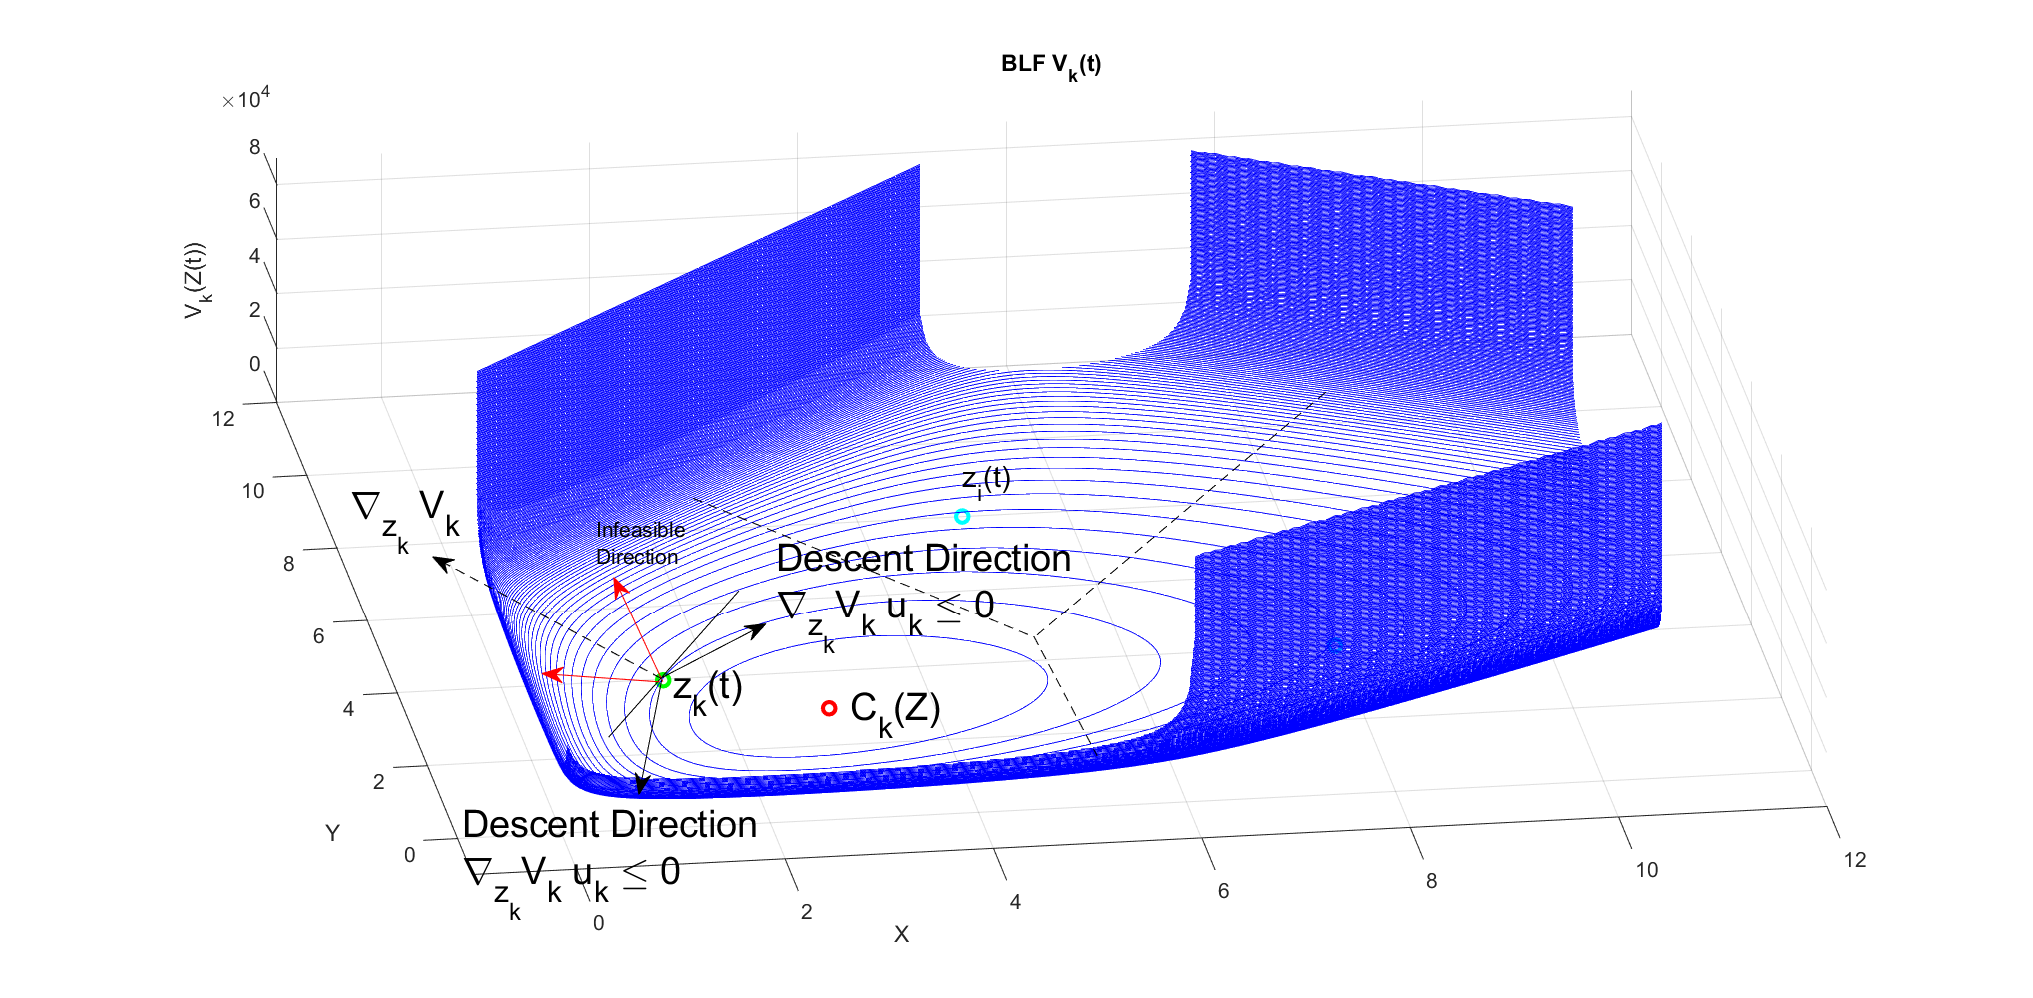
\includegraphics[width=1\linewidth]{BLF_3D_Contour_zoom}
	\caption{Barrier Lyapunov Function and The Feasible Direction of Agent $k$}
	\label{fig:Contour_3D}
\end{figure}

\noindent Figure \ref{fig:Contour_3D} demonstrates the concept of Proposition 2, there exists a feasible movement that ensures the state constraint. \\

\noindent \textbf{Proof.} \\
From the initial condition, agent $k$ and the center of Voronoi partition $C_k$ is inside the coverage region so the BLF is well defined. Because the proposed function is differentiable, the directional derivative delivers a descent and ascent direction of $V_k{Z}$ related to the variable $z_k$. Since the region $\interior Q$ is convex and the BLF is designed so that it always has a local optimum at $C_k$, it implies that $z_k$ is feasible if it follows the descent direction.

\noindent Due to the complexity of this problem, we must analyze all of the necessary and sufficient conditions to ensure the feasibility for all agents. This will be presented with more details in the Discussion in chapter 5. \\

\noindent According to the proposition 2, we analyze $\frac{\partial V_k(Z)}{dz_k}\dot z_k$ to obtain a control law for agent $k$

\begin{equation} \notag
\begin{split}
%V_k(Z) & = \displaystyle\sum_{j=1}^{m} [ln(\frac{b_j - a_{jx}C_{kx} - a_{jy}C_{ky}}{b_j - a_{jx}z_{kx} - a_{jy}z_{ky}})]^2 \\
& \frac{\partial V_k(Z)}{dz_k}\dot z_k \\
& = \frac{\partial V_k(Z)}{dz_{kx}}\dot z_{kx} + \frac{\partial V_k(Z)}{dz_{ky}}\dot z_{ky} \\
& = \dot z_{kx} \displaystyle\sum_{j=1}^{m} \frac{\partial}{\partial z_{kx}} [ln(\frac{b_j - a_{jx}C_{kx} - a_{jy}C_{ky}}{b_j - a_{jx}z_{kx} - a_{jy}z_{ky}})]^2 + \dot z_{ky} \displaystyle\sum_{j=1}^{m} \frac{\partial}{\partial z_{ky}} [ln(\frac{b_j - a_{jx}C_{kx} - a_{jy}C_{ky}}{b_j - a_{jx}z_{kx} - a_{jy}z_{ky}})]^2 \\
%
& = \displaystyle\sum_{j=1}^{m} 2ln(\frac{b_j - a_{jx}C_{kx} - a_{jy}C_{ky}(t)}{b_j - a_{jx}z_{kx} - a_{jy}z_{ky}})(\frac{-a_{jx}\frac{\partial C_{kx}}{\partial z_{kx}}\dot z_{kx} - a_{jy}\frac{\partial C_{ky}}{\partial z_{kx}}\dot z_{ky}}{b_j - a_{jx}C_{kx} - a_{jy}C_{ky}} + \frac{-a_{jx}\dot z_{kx} - a_{jy}\dot z_{ky}\dot z_{ky}}{b_j - a_{jx}z_{kx} - a_{jy}z_{ky}}) \\ 
\end{split}
\end{equation}

\noindent Substitute the partial derivative of virtual mass ${z_k}$ from (\ref{vm_derivatve}) into ${\dot V(Z)}$, we obtain
\begin{equation} \notag
\begin{split}
&\frac{\partial V_k(Z)}{dz_k}\dot z_k = -\mu_k(\psi_{k})\frac{v_k}{\norm{w_{k_0}}}. \\
&\underbrace{cos(\psi_{k}) \displaystyle\sum_{j=1}^{m} 2ln(\frac{b_j - a_{jx}C_{kx} - a_{jy}C_{ky}}{b_j - a_{jx}z_{kx} - a_{jy}z_{ky}})(\frac{a_{jx}cos(\theta_{k}) + a_{jy}sin(\theta_{k})}{b_j - a_{jx}z_{kx} - a_{jy}z_{ky}} - \frac{a_{jx}\frac{\partial C_{kx}}{\partial z_{kx}}cos(\theta_{k}) + a_{jy}\frac{\partial C_{ky}}{\partial z_{kx}}sin(\theta_{k})}{b_j - a_{jx}C_{kx} - a_{jy}C_{ky}})}_{M_k(t)}
\end{split}
\end{equation}

\noindent The complicated $M_k(t)$ can be obtained by the full state feedback at time t, which are ${z_k(t), \theta_{k}(t), C_k(t)}$ and constant $A \txtspc{,} b$. Note that the gradient $ [\frac{\partial C_{kx}}{\partial z_{kx}} \txtspc{ } \frac{\partial C_{ky}}{\partial z_{ky}}] $ is complicated but there already exists an analytical formulation. These terms will be introduced later in the controller design section. We obtain
\begin{equation} \label{time_derivative_BLF}
\begin{split}
\frac{\partial V_k(Z)}{dz_k} &  = -\mu_k(t)\frac{v_k}{\norm{w_{k_0}}} M_k(t)\\
\end{split}
\end{equation}

\noindent \textbf{Intuitive Explanation of the Switching Control Law:} \\
Note that we have two Lyapunov functions in our derivation, which are ${H(Z(t))}$ and ${V(Z(t))}$. While the negative time derivative of $H(Z(t))$ ensures the asymptotic stability of the coverage control, it does not reflect the feasibility of the state. On the other hand, from proposition 2, there exist a feasible movement of agent $z_k$, but does not guarantee asymptotic stability of coverage control because its time derivative is not always non-positive. \\
The idea behind is to use the property of Proposition 2 that whenever $\frac{\partial V_k(Z)}{dz_k}\dot z_k \leq 0$, ${z_k \in \interior{Q}}$, the virtual mass ${z_k}$ is allowed to move. As long as there exists a control input with a positive control gain ${\mu_k}$ that satisfies this condition, it is shown that ${\dot H(Z(t)) < 0}$ and the coverage control converge asymptotically. \\
Additionally, ${\mu_k \in \mathbb{R}_+}$ must satisfy the condition obtained from section 3.2 to handle the input saturation. \\
\textbf{Proposition 3:} \\
The following switching condition ensures that all agents' virtual mass always stay inside the interior of region Q and asymptotically converge to the set of centroidal Voronoi configuration. \\ 
\begin{equation} \label{switching_law}
\begin{split} 
\mu_k(t) = \twopartdef {\mu_k(t) \in \mathbb{R}_+} {, M_k(t) \geq 0} {0} {, M_k(t) < 0}
\end{split}
\end{equation}
\noindent \textbf{Proof.} \\
$\bullet$ \textbf{\textit{Feasibility of States}} \\
\noindent \underline{${M_k(t) \geq 0 \implies \mu_k(t) \in \mathbb{R}_+}$} \\
\begin{equation} \notag
\begin{split} 
\frac{\partial V_k(Z)}{dz_k} & = -\mu_k(t)\frac{v_k}{\norm{w_{k_0}}} M_k(t) \\
& = -\norm{\mu_k(t)}\frac{v_k}{\norm{w_{k_0}}} \norm{M_k(t)} \leq 0 \\
\text{Proposition 2} \implies & z_k(t) \in \interior Q \txtspc{as} t \rightarrow \infty 
\end{split}
\end{equation}

\noindent \underline{${M_k(t) < 0  \implies \mu_k(t) = 0}$} 
\[\exists t \in [t_0 \txtspc{ } \infty) \txtspc{ } z_k(t) \in \interior{Q}\]
\[\mu_k(t) = 0 \implies \dot z_k(t) = 0 \implies z_k(t + \delta t) = z_k(t) \in \interior{Q} \txtspc{ } for \txtspc{ } \delta t \rightarrow 0\]
Intuitively, if the virtual mass of an agent is not allowed to move due to state feasibility, the control input forces it to stay there by keep the agent rotate at the current virtual mass. \\

\noindent (\ref{switching_law}) fulfills state constraints (q.e.d). \\

\noindent $\bullet$ \textbf{\textit{Asymptotic Convergence of Virtual Masses on Centroidal Voronoi Configuration}} \\
\noindent \underline{${M_k(t) \geq 0 \implies \mu_k(t) \in \mathbb{R}_+}$} \\
\[\mu_k(t) \in \mathbb{R}_+ \implies \dot H(Z) = - \displaystyle\sum_{k=1}^{n} \frac{\mu_k(\psi_{k})M_{V_{k}}v_{k}}{\norm{w_{0}}\norm{z_{k} - C_{V_{k}}}} \langle{z_{k} - C_{V_{k}},e^{i\theta_{k}}}\rangle^{2} \leq 0\] 
From Proposition 1: LaSalle' invariance principle implies that system approaches the unique stable equilibrium points if and only if ${z_{k} = C_{V_{k}} \forall k \in \{1,...,n\}}$ \\

\noindent \underline{${M_k(t) < 0  \implies \mu_k(t) = 0}$} \\
Assume model's dynamic approaches the set of stable equilibrium points at time ${t \in [t_0 \txtspc{ } \infty)}$ \\
This set is defined as ${\Omega = \{Z \in \interior Q| \dot H(Z(t')) = 0 \txtspc{ } \forall t' \in [t \txtspc{ } \infty)\}}$. We have
\[\dot H(Z(t')) = 0 \txtspc{ } \forall t' \in [t \txtspc{ } \infty)\]
\[\Leftrightarrow \mu_k(t') = 0 \txtspc{ } \forall k \in \{1,...,n\} \txtspc{ } \forall t' \in [t \txtspc{ } \infty) \]
\[\Leftrightarrow M_k(t') < 0 \txtspc{ } \forall k \in \{1,...,n\} \txtspc{ } \forall t' \in [t \txtspc{ } \infty) \tag{P3.1} \] 

\noindent If every agent rotates around its unchanged virtual mass, the center of each Voronoi cell remains constant \\
\[\mu_k(t') = 0 \implies \dot z_k(t') = 0 \implies z_k(t') = z_k(t) \txtspc{ } \forall k \in \{1,...,n\} \txtspc{ } \forall t' \in [t \txtspc{ } \infty)\]
\[\implies C_k(t') = C_k(t) = const  \txtspc{ } \forall k \in \{1,...,n\} \txtspc{ } \forall t' \in [t \txtspc{ } \infty)\]

\noindent Then from the definition, $\psi_{k}$ has the same dynamic with ${\theta_{k}}$\\
\[\mu_k(t') = 0 \implies u_{k}(t') = w_{k_0} \txtspc{ } \text{from (\ref{control_with_consraint})} \txtspc{ } \forall t' \in [t \txtspc{ } \infty)\]
\[\psi_{k} = \angle (z_{k} - C_{V_{k}}, v_{k}e^{i\theta_{k}}) \txtspc{,} C_k(t') = const \txtspc{,} \dot z_k(t) = 0 \implies \dot \psi_{k} = \dot \theta_{k} = w_{k_0}\]

\noindent It is shown that if these equilibrium points are not the CVT by the following contradiction
\[\dot \psi_{k} = w_{k_0} \implies \exists t' \in [t \txtspc{ } \infty): cos(\psi_{k}(t')) = 0 \]
\[\implies \exists t' \in [t \txtspc{ } \infty): M_k(t') = 0\]

\noindent This contradicts the statement (P3.1) and consequently these equilibrium points are unstable. Only when the virtual masses of every agent coincide the set of centroidal Voronoi configuration, ${H(Z) = 0 \txtspc{,} \dot H(Z) = 0}$. The theorem of Barbashin states that the system is asymptotic stable. (q.e.d)

\section{Controller Design}
\subsection{Scaling Factor for Input Saturation}
In \textbf{Proposition 1} (Subsection 3.2. Problem of Input Constraints) we pointed out the existence of an feasible positive control gain ${\mu_k(\psi_{k})}$. The following derivation determines ${\mu_k(\psi_{k}): [0 \txtspc{ } 2\pi] \rightarrow \mathbb{R}_+}$ in detail. \\
% PROBLEM STATEMENT **************************************************************************************************************************************************
$\bullet$ \textbf{Problem statement}\\
For a given reference ${C_{V_{k}} = [C_{kx} \txtspc{ } C_{ky}]^{T} \in \mathbb{R}^{2}}$, upper and lower input saturation ${U_{up}, U_{low} > 0}$, desired orbiting velocity ${w_{k_0}\in [-U_{low} \txtspc{ } U_{up}]}$. From the measurement of virtual mass's current position ${z_{k} = [z_{kx} \txtspc{ } z_{ky}]^{T} \in \mathbb{R}^{2}}$ and heading orientation  ${\theta_{k} \in [0, 2\pi]}$. By defining ${\psi_{k} = \angle (z_{k} - C_{V_{k}}, v_{k}e^{i\theta_{k}}) \in [0 \txtspc{ } 2\pi]}$, find ${\mu_k(\psi_{k}): [0 \txtspc{ } 2\pi] \rightarrow \mathbb{R}_+}$ to keep the control input ${u_{k} = w_{k_0} + \mu_k(\psi_{k})sign(w_{k_0})cos(\psi_{k})}$ always stay in feasible region, which means ${u_{k} \in [-U_{low} \txtspc{ } U_{up}]}$. \\
Task: Find
\begin{equation} \notag
\begin{split}
&\mu_k(\psi_{k}) \in \mathbb{R}_+ \txtspc{,} \forall \psi_{k} \in [0 \txtspc{ } 2\pi]\\
\end{split}
\end{equation}
so that 
\begin{equation}
\begin{split}
& u_{k} = w_{k_0} + \mu_{k}(\psi_{k})sign(w_{k_0})cos(\psi_{k}) \\
& u_k \in [-U_{low} \txtspc{ } U_{up}] \txtspc{,} \forall \psi_{k} \in [0 \txtspc{ } 2\pi] \\
\end{split}
\end{equation}
% SOLUTION **************************************************************************************************************************************************
\noindent $\bullet$ \textbf{Solution} \\
\noindent For any ${C_{V_{k}}}$, a desired orbiting angular velocity is ${w_{k_0}}$ known in advance. From these factors, we propose a control gain that depends from actual ${\psi_{k}}$ and ${w_{k_0}}$ as following \\

\indent $\blacksquare$ If ${w_{k_0} > 0}$ 
\begin{equation} \label{adaptive_gain_positive_w0} %***************************************************
\begin{split}
& \mu_k(\psi_{k})sign(w_{k_0}) \\
& = \mu_k(\psi_{k})\\
& = \twopartdef {k_1 \in \mathbb{R} \txtspc{,} 0 < k_1 \leq U_{up} - \norm{w_{k_0}}} 		{for ${ }$ \psi_{k} \in [\frac{\pi}{2} \txtspc{ } \frac{3\pi}{2}]} 
				{k_2 \in \mathbb{R} \txtspc{,} 0 < k_2 \leq U_{low} + \norm{w_{k_0}}} 		{for ${ }$ \psi_{k} \in [0 \txtspc{ } \frac{\pi}{2}] \cup [\frac{3\pi}{2} \txtspc{ } 2\pi]} \\
\end{split}
\end{equation}
%
\indent $\blacksquare$ If ${w_{k_0} < 0}$ 
\begin{equation} \label{adaptive_gain_negative_w0} %***************************************************
\begin{split}
& \mu_k(\psi_{k})sign(w_{k_0}) \\
& = -\mu_k(\psi_{k})\\
& = \twopartdef {-k_1 \in \mathbb{R} \txtspc{,} 0 < k_1 \leq U_{low} - \norm{w_{k_0}}} 		{for ${ }$ \psi_{k} \in [\frac{\pi}{2}\txtspc{ } \frac{3\pi}{2}]} 
				{-k_2 \in \mathbb{R} \txtspc{,} 0 < k_2 \leq U_{up} + \norm{w_{k_0}}}			{for ${ }$ \psi_{k} \in [0\txtspc{ } \frac{\pi}{2}] \cup [\frac{3\pi}{2}\txtspc{ } 2\pi]} \\
\end{split}
\end{equation}

% SOLUTION **************************************************************************************************************************************************
\noindent $\bullet$ \textbf{Proof.} The feasibility of control input\\
\indent $\blacksquare$ For predefined ${w_{k_0} > 0}$ 
\begin{equation} \notag %\label{Proof_positive_adaptive_gain} %***************************************************
\begin{split}
u_{k} & = w_{k_0} + \mu_k(\psi_{k})sign(w_{k_0})cos(\psi_{k})\\
& = \norm{w_{k_0}} + \mu_k(\psi_{k})cos(\psi_{k})  \\
(\ref*{adaptive_gain_positive_w0}) \implies & \twopartdef {u_{k} = \norm{w_{k_0}} + k_1cos(\psi_{k})} {for \txtspc{ } 0 < k_1 \leq U_{up} - \norm{w_{k_0}} \txtspc{,}\psi_{k} \in [\frac{\pi}{2}  \txtspc{ } \frac{3\pi}{2}]}
{u_{k} = \norm{w_{k_0}} + k_2cos(\psi_{k})} {for \txtspc{ } 0 < k_2 \leq U_{low} + \norm{w_{k_0}} \txtspc{,} \psi_{k} \in [0 \txtspc{ } \frac{\pi}{2}] \cup [\frac{3\pi}{2}\txtspc{ } 2\pi]}\\
\implies & \twopartdef {u_{k} \leq \norm{w_{k_0}} + (U_{up} -\norm{w_{k_0}})} {for ${ }$ \psi_{k} \in [\frac{\pi}{2} \txtspc{ } \frac{3\pi}{2}]} {u_{k} \geq \norm{w_{k_0}} + (U_{low} + \norm{w_{k_0}})}   {for ${ }$ \psi_{k} \in [0 \txtspc{ } \frac{\pi}{2}] \cup [\frac{3\pi}{2} \txtspc{ } 2\pi]} \\
\implies & u_{k} \in [-U_{low} \txtspc{ } U_{up}] \txtspc{ } \forall \psi_{k} \in [0 \txtspc{ } 2\pi] (q.e.d) \\
\end{split}
\end{equation}

\indent $\blacksquare$ Analog for ${w_{k_0} < 0}$ 
\begin{equation} \notag %\label{Proof_positive_adaptive_gain} %***************************************************
\begin{split}
u_{k} & = w_{k_0} + \mu_k(\psi_{k})sign(w_{k_0})cos(\psi_{k})\\
& = -\norm{w_{k_0}} - \mu_k(\psi_{k})cos(\psi_{k})  \\
(\ref*{adaptive_gain_negative_w0}) \implies & \twopartdef {u_{k} = -\norm{w_{k_0}} - k_1cos(\psi_{k})} {for \txtspc{ } 0 < k_1 \leq U_{low} - \norm{w_{k_0}} \txtspc{,}\psi_{k} \in [\frac{\pi}{2}  \txtspc{ } \frac{3\pi}{2}]} 
{u_{k} = -\norm{w_{k_0}} - k_2cos(\psi_{k})} {for \txtspc{ } 0 < k_2 \leq U_{up} + \norm{w_{k_0}} \txtspc{,} \psi_{k} \in [0 \txtspc{ } \frac{\pi}{2}] \cup [\frac{3\pi}{2}\txtspc{ } 2\pi]}\\
\implies & \twopartdef {u_{k} \geq -\norm{w_{k_0}} - (U_{low} -\norm{w_{k_0}})} {for ${ }$ \psi_{k} \in [\frac{\pi}{2} \txtspc{ } \frac{3\pi}{2}]} {u_{k} \leq -\norm{w_{k_0}} + (U_{up} + \norm{w_{k_0}})}   {for ${ }$ \psi_{k} \in [0 \txtspc{ } \frac{\pi}{2}] \cup [\frac{3\pi}{2} \txtspc{ } 2\pi]} \\
\implies & u_{k} \in [-U_{low} \txtspc{ } U_{up}] \txtspc{ } \forall \psi_{k} \in [0 \txtspc{ } 2\pi] (q.e.d) \\
\end{split}
\end{equation}

\subsection{Model Based Control Design for State Constraint}
Recall
\begin{equation} \label{M_k}
\begin{split}
M_k(t) = & cos(\psi_{k}) \displaystyle\sum_{j=1}^{m} 2ln(\frac{b_j - a_{jx}C_{kx} - a_{jy}C_{ky}}{b_j - a_{jx}z_{kx} - a_{jy}z_{ky}})\\
& \txtspc{    } (\frac{a_{jx}cos(\theta_{k}) + a_{jy}sin(\theta_{k})}{b_j - a_{jx}z_{kx} - a_{jy}z_{ky}} - \frac{a_{jx}\frac{\partial C_{kx}}{\partial z_{kx}}cos(\theta_{k}) + a_{jy}\frac{\partial C_{ky}}{\partial z_{kx}}sin(\theta_{k})}{b_j - a_{jx}C_{kx} - a_{jy}C_{ky}})
\end{split}
\end{equation}
The switching controller law from (\ref{switching_law}) is used to consider whether each agent moves or rotates around its virtual mass through the control gain as follows 
\[\mu_k(t) = \twopartdef {\mu_k(t) \in \mathbb{R}_+} {M_k(t) \geq 0} {0} {M_k(t) < 0}\]

\noindent In [5], Appendix A, Lee already formulated the gradient of $C_k = [\frac{\partial C_{kx}}{\partial z_{kx}} \txtspc{ } \frac{\partial C_{ky}}{\partial z_{ky}}]$ as \\
\begin{equation} \label{grad_C}
\frac{\partial {C}^{(a)}_k}{\partial {z}^{(b)}_k} = \frac{(\int_{\partial V_{i,j}}^{} \phi(q)q^{(a)} \frac{q^{(b)} - {z}^{(b)}_k}{\norm{z_j - z_i}} dq)}{m_k} - \frac{(\int_{\partial V_{i,j}}^{} \phi(q)\frac{q^{(b)} - {z_k}^{(b)}}{\norm{z_j - z_i}} dq)(\int_{V_k(Z)}^{} \phi(q)q^{(a)}dq)}{m^2_k}
\end{equation}
where $a,b \in {x,y}$ and $m_k = \int_{V_k(Z)}^{} \phi(q)dq$. \\
With all of the necessary state feedback, the implementation of a controller for ${k-th}$ agent is presented as follows

\begin{algorithm} [H] % enter the algorithm environment
	\caption{Computation of Control Input for n agents} % give the algorithm a caption
	\label{alg1} % and a label for \ref{} commands later in the document
	\textbf{Data:}\\
	- Information of dominating region ${Q}$: ${A \in \mathbb{R}^{m \times 2} \txtspc{,} b \in \mathbb{R}^m }$. \\
	- Input limits: ${[-U_{k_{low}} \txtspc{ } U_{k_{up}}] \txtspc{,} \forall k \txtspc{,} U_{k_{low}},U_{k_{up}} > 0}$ \\
	- Desired orbiting velocity: ${w_{k_0} \in [-U_{k_{low}} \txtspc{ } U_{k_{up}}]}$ \\
	- Constant heading velocity: ${v_k \in \mathbb{R}_+}$ \\
	\textbf{Result:} \\
	- Control input for each agent: ${u_k}$ \\
	\noindent\rule{\textwidth}{1pt}

	$\bullet$ \textbf{Initialization} \\% // Do once \\
	- Choose feasible control gain: (\ref{adaptive_gain_positive_w0}),(\ref{adaptive_gain_negative_w0}) ${\implies}$  ${\mu_k \in \{k_1,k_2\} \txtspc{ } \forall{k} \in \{1,...,n\}}$ \\
	- Initialize all agents position that satisfy: ${z_k(t_0) \in \interior{Q} \txtspc{ } \forall{k} \in \{1,...,n\}}$ \\
	
	$\bullet$ \textbf{Loop}% // Execution
	\begin{algorithmic} % enter the algorithmic environment
	\FOR{k = 1 \TO n } 
		\STATE { } 
		\STATE {${\psi_{k} \leftarrow arccos(\frac{\langle{z_{k} - C_{V_{k}}},{e^{i\theta_{k}}}\rangle}{\norm{z_{k} - C_{V_{k}}}})}$} 
		\STATE { } 
		\IF{${\psi_{k} \in [\frac{\pi}{2} \txtspc{ } \frac{3\pi}{2}]}$} 
			\STATE {${\mu_k \leftarrow k_1}$} 
		\ELSE 
			\STATE {${\mu_k \leftarrow k_2}$} 
		\ENDIF
		\STATE { } 

		\STATE {${(\frac{\partial C_{kx}}{\partial z_{kx}} \txtspc{  } \frac{\partial C_{ky}}{\partial z_{ky}}) \leftarrow (\ref{grad_C})}$} 
		\STATE { } 
		
		\STATE {${M_k  \leftarrow (\ref{M_k})}$} 
	
		\IF{${M_k \geq 0}$} 
			\STATE {${\mu_k \leftarrow \mu_k}$} 
		\ELSE 
			\STATE {${\mu_k \leftarrow 0}$} 
		\ENDIF
		
		\STATE { } 

		\STATE {${u_k \leftarrow w_{k_0} + \mu_k sign(w_{k_0})cos(\psi_{k})}$} 
	\ENDFOR	
	\end{algorithmic} % enter the algorithmic environment	
	\textbf{Return:} ${u_k \txtspc{ } \forall k \in \{1,...,n\}}$\\
\end{algorithm}




